\chapter{Exercise 2}
In exercise 2 the task was to implement unit tests for the class Line, which represents the linear regression of multiple points. In the following every test is looked at and some explanation is given on why this test was choosen. The full source code can be found at \ref{lst:linetest}.

\section{Testcases and description}

\subsection{Constructor}
As defined in the exercise two contructors should be created, a default constructor that creates an empty line with no points and a parametrized one, that initializes the line with given points. For this three test cases were written.

\begin{enumerate}
    \item empty line with default constructor \\
    This test calls the default constructor and checks if an empty line is created by asserting the length equals zero.
    \item initialized line with points \\
    This test calls the parametrized constructor with an array of three points and checks if the line is correctly initialized by checking if line.lentgh() returns three.
    \item empty line with empty points array \\
    This test checks if the parametrized constructor creates an empty line if it is called with an empty array of points. This was done to validate that the internal structure can handle empty arrays and does not crash or throw exceptions.
\end{enumerate}

\subsection{Line.add}
The add method should add a given point to the line. To validate the functionality two cases were checked.

\begin{enumerate}
    \item add additional point to line \\
    This test checks the most common use of add. It appends one point to an existing empty line and validates, if the point is added by checking if the length is incremented. 
    \item add null to line \\
    This test validates an edge case, where instead of a point the value null is given as a parameter. This should not crash or throw any NullPointerExceptions and just not add any points to the line. This was again validated by checking the length of the line after adding null.
\end{enumerate}

\subsection{Line.length}
The method length() should return the current length of the line as an integer. To validate this behaviour two test was created.

\begin{enumerate}
    \item length is created with correct length \\
    This test checks to basic functionality of length(). For this a line with three points is created, then the length method is called to check if it returns three.
    \item length increments when adding points on runtime \\
    For this test an empty line is created and a single point is added. This should increment the length of the line by one. This was done to check if length is updated when a line is edited dynamically and is not set statically on creation.
\end{enumerate}

\subsection{Line.equals}
\label{sec:line_equals}
To test the equals method seven different cases were looked at. This amount comes from the different specifications, which were written in the exercise.

\begin{enumerate}
    \item lines are not equal with different points \\
    There are two behaviours for the equals method. Two lines, that do not have the same points should be considered as not equal, so Line.equals()should return false. For this two lines with different points were created and checked if equals returns false as defined.
    \item lines with same points in different orders \\
    As the exercise states, lines with the same points, independent of the order should be considered as equal to each other. To check this behaviour the test creates two lines, one with the points ((0,0),(0,1),(0,2)) and one with the points ((0,2),(0,0),(0,1)). These lines should be considered as equal to each other which was asserted.
    \item object equals itself \\
    As one would assume, the equals method should return true when called with the same object. This was tested by creating a line and checking if it equals itself. The major reason for this test was checking if the comparison may change something while evaluating the object. This should not happen and is checked by this test.
    \item lines should not be equal when different with multiple points in line \\
    This test is a bit more complicated. Two lines, that are the same length, but with different points should not be equal. Also, the equals algorithm should deal with points double in line and not confuse them as beeing equal. For this two lines where created, one with the points ((0,0),(0,0)) and one with the points ((0,0),(0,1)). These two lines should not be equal. Depending on the implementation, the fact that one point is twice in one line can break the algorithm. To validate that the used implementation is safe this test was written.
    \item lines with different length should not be equal \\
    This test generates two lines, one with length 0 and one with length 3. Those two lines should not be equal. This test was choosen to check if length is tested, which should be that case and is faster then checking every point in one line.
    \item line should not be equal with null \\
    To check if equals can cope with null as an input without throwing a NullPointerException, this test calls equals on a line with length 0 and compares it to null.
    \item lines with points (A,A,B) and (B,B,A) should not be equal \\
    The idea for this test came when debugging the line class. The choosen implementation did not work correctly in cases where lines l1 ((0,0),(0,0),(1,1)) and l2 ((0,0),(1,1),(1,1)) were compared. Even though this lines should not be equal, the equals method returned true and assumed they were equal. To check that this misbehaviour was fixed and stays fixed during further development this testcase was implemented.
\end{enumerate}

\subsection{Line.hashCode}
As the exercise states, hashCode must be implemented in a suitable manner. According to the API documentation for Object.hashCode this means that the following specifications must be fulfilled\footnote{\url{https://docs.oracle.com/javase/7/docs/api/java/lang/Object.html#hashCode()}}.
\begin{itemize}
    \item Whenever it is invoked on the same object more than once during an execution of a Java application, the hashCode method must consistently return the same integer, provided no information used in equals comparisons on the object is modified. This integer need not remain consistent from one execution of an application to another execution of the same application.
    \item If two objects are equal according to the equals(Object) method, then calling the hashCode method on each of the two objects must produce the same integer result.
    \item It is not required that if two objects are unequal according to the equals(obj) method, then calling the hashCode method on each of the two objects must produce distinct integer results. However, the programmer should be aware that producing distinct integer results for unequal objects may improve the performance of hash tables.
\end{itemize}

To check these specifications three tests were written.
\begin{enumerate}
    \item \textbf{testTwoLinesHaveSameHashCodeSameOrder} \\
    This test check if two lines with the same points in the same order have the same hashCode. As stated in the exercise such lines should be considered equal and should produce the same hashCode (see definitions from Java Api).
    \item \textbf{testTwoLinesHaveSameHashCodeDifferentOrder} \\
    Lines with only the order scrambled should be considered equal. This behaviour is validated with tests in \ref{sec:line_equals}. According to the Java API documentation such lines should return the same hashCode. This test is pretty similar to the test before, but validates that hashCode does work with different ordered lines.
    \item \textbf{testHashCodeStaysSameForMultipleCalls} \\
    As stated in the Java API: " Whenever it is invoked on the same object more than once during an execution of a Java application, the hashCode method must consistently return the same integer". This means as long as the JVM stays the same and the object is not manipulated on a field that is used to evaluate equality of this object it \textbf{must} produce the same hashCode. This is tested by calling hashCode twice on the same line object and validating that the result stays the same. This also checks if the hashCode is calculated with no degree of randomness that is based on for example a timestamp.
\end{enumerate}

\subsection{Line.toString()}
Since the output format for a line was specified in the exercise, the toString method had to be overridden. To check the correct return value three testcases were considered, as there were three possible outputs.
\begin{enumerate}
    \item \textbf{testToStringEmptyLine} \\
    The first output is for empty lines. This was not defined in the exercise, so it was assumed, that simple () should be returned. This was tested by creating a an empty line and asserting if toString would return (). This was the most sensible approach, since the toString method should returnm a list of all points, which are none for an empty line. 
    \item \textbf{testToStringOnePoint} \\
    The second testcase was to check, if a line with length = 1 gives the correct return value. This was done by creating an empty line and adding one point. The main purpose of this test was to check wether the seperators between each point is printed correctly. As there is only one point, there shouldn't be any seperators before or after the point. The output is assumed to be ((Point.x, Point.y)).
    \item \textbf{testToStringWithThreePointsInLine} \\
    This is the most common case. In this test multiple points are used to create the line. This shows the full output for a single line, with seperators between the points and no seperation for the last point. The corresponding output is build with String.format, since it is assumed that Point.toString() works as defined.
\end{enumerate}

\subsection{Line.isValid}
Up until now, the line was just an Array of points, without linear regression. The following methods are all used to calculate the corresponding line represented by the given points. The first method checks if a line is valid, for this the following  definitions where used.

\begin{itemize}
    \item A line is invalid with less then or equal to one point.
    \item A line is invalid if the slope can not be calculated.
    \item A mline is invalid if the intercept can not be calculated.
    \item A line is valid in all other cases
\end{itemize}

To test these definitions, three tests where used
\begin{enumerate}
    \item \textbf{testIsInvalidWhenZeroPointsAreStored} \\
    As stated a line is invalid with less then one point, so it is tested if an empty line is invalid.
    \item \textbf{testIsInvalidWhenSlopeOrInterceptCanNotBeCalculated} \\
    This test validated wether a line is invalid if its slope or intercept can not be calculated. This is done by creating a line with three points, all of which are parallel to the y-axsis. Since neither the slope nor the intercept can be calculated in this case, one test validates both definitions. As this is true for all lines, this test validates the whole behaviour.
    \item \textbf{testLineIsValid} \\
    The last case tests if the line can be valid at all by initializing a line where one can calculate slope and intercept and that has more then 2 points (in this case three points with a slope of 1 and an intercept of 0).
\end{enumerate}

\subsection{Line.slope}
The method slope is defined to calculate the slope of any valid line using linear regression. Also, if the slope could not be calculated the method shall throw an RegressionFailedException. This is tested with four tests.
\begin{enumerate}
    \item \textbf{testReturnsCorrectSlopeForLine} \\
    In this case it is tested, if a correct calulation is done for three points that are all on a 45 degree angled line. (maybe instert figutre here / reference). The slope of this line is asserted to be 1.0
    \item \textbf{testReturnsCorrectSlopeForSixPoints} \\
    This test is used to check wetehr the calculation for slope is dependend on the points beeing in a straight line. In this case the points are one the x or y axis respectively and the slope was calculated with WolframAlpha\footnote{\url{https://www.wolframalpha.com/input/?i=linear((1,0),(3,0),(5,0),(0,1),(0,3),(0,5))}}
    \item \textbf{testThrowsExceptionWhenSlopeNotCalculable} \\
    This test validates if a RegressionFailedException is thrown, when the line is invalid or the calculation for slope fails for any kind of reason (f.e. division by 0). For this a Line is created where all points are parallel to the y axis. Its is not possible (at least with linear regression) to calculate the slope, so this should throw an RegressionFailedException. This is asserted with \lstinline[language=java]{assertThrows(RegressionFailedException.class, () => l1.slope()}, which can be used since the Unittests where implemented with JUnit 5.
    \item \textbf{testAddPointsOtherSlope} \\
    The last text is used to check the caching behaviour of slope. The result shall be stored after the first calculation and only changed ones the line is manipulated. For this a line is created the slope ist calculated and then points are added to the line. After that its asserted that the slope changed and is not return from the stored cache.
\end{enumerate}

\subsection{Line.intercept}
The last method for the class Line is intercept, which calculates the y-axis intercept of a line. Like with slope, intercept can only be calculated with a valid line. To test if intercept handles the calculation correctly, four tests where written
\begin{enumerate}
    \item \textbf{testInterceptReturnsCorrectValue} \\
    The first test is the most common one. It is expected that when creating a line the intercept is calculated correctly with linear regression. This is tested by creating a line l1 with ((0,1),(1,2)) and asserting that intercept returns 1.0.
    \item \textbf{testInterceptReturnsCorrectValueForLargerLines} \\
    As for slope a longer line was choosen where not all points are straight on the line. The intercept was calculated with WolframAlpha again. The biggest difference to most other testcases is that we assert within some Accuracy, which is needed as double opertations in Java are not 100\% accurate by the nature of the way they are handled.
    \item \textbf{testInterceptThrowsExceptionWhenNotCalculable} \\
    Like with slope intercept should throw a RegressionFailedException when the line is not valid or any other arithmetic problem happens. This is checked by creating a line parallel to the y-axis and asserting that intercept throws a RegressionFailedException. As in Slope this is done by \lstinline[language=java]{assertThrows(...)}.
    \item \textbf{testInterceptWithNaNforValidLine} \\
    The last test checks how well intercept and the class Line handles NaN as point values. Since multiple tests for Double.NaN was already tested in Point to not crash at any operation, this is done for intercept.
\end{enumerate}

\section{Testresults and coverage}

The following screenshots show the results (see \ref{fig:test_results}) when running the test suite and the coverage (see \ref{fig:test_cov}) produced with the selected tests. As seen the coverage is not 100\%, which should be reached as best as possible. The problem comes form the implementation of intercept() (see \ref{fig:missing_cov}). The method internally calls slope() which, when it fails, will throw an RegressionFailedException, which will be thrown further up the call stack to the test. After the internal slope() call, the method calculates the y-axis intercept and checks, if the calculation was sucessful. This is done to handle values like Double.NaN correclty. Since slope() already checks this behaviour, the test can't reach this code and can't cover it. 

\begin{figure}[h!]
    \begin{center}
        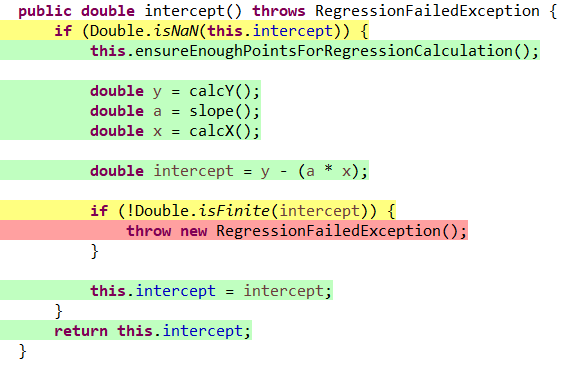
\includegraphics{img/missingcov.png}
        \caption{Missing coverage in Line.intercept due to unreachable code}
        \label{fig:missing_cov}
    \end{center}
\end{figure}

\begin{figure}[p!]
    \begin{center}
        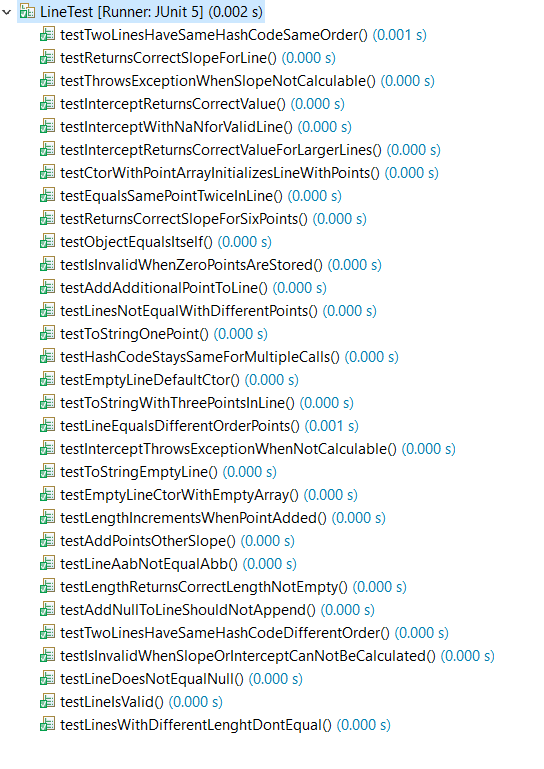
\includegraphics{img/testresults.png}
        \caption{Testresults for LineTest, all tests are passed}
        \label{fig:test_results}
    \end{center}
\end{figure}

\begin{figure}[p!]
    \begin{center}
        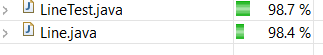
\includegraphics{img/testcoverage.png}
        \caption{Coverage produced by LineTest for class Line, not 100\% coverage}
        \label{fig:test_cov}
       \end{center}
\end{figure}
